
\section{Results}

\begin{frame}{Results}
  
  Revisiting the model
  $$\begin{cases}
    \begin{array}{rl}
      dM\hspace{-.8em}&=[aMC - \frac{gM(t-\tau)}{1-C(t-\tau)} + \gamma M (1-M-C)]dt+\beta M(1-M)dW,\\
      dC\hspace{-.8em}&=[rC(1-M-C) - dC - aMC]dt.\\
    \end{array}
    \end{cases}$$\\
  We are interested in the effects of:
  \begin{itemize}
  \item the initial condition\\
  \item beta\\
  \item tau\\
  \end{itemize}
  

\end{frame}

\begin{frame}{Initial Conditions}
Add arc to graph
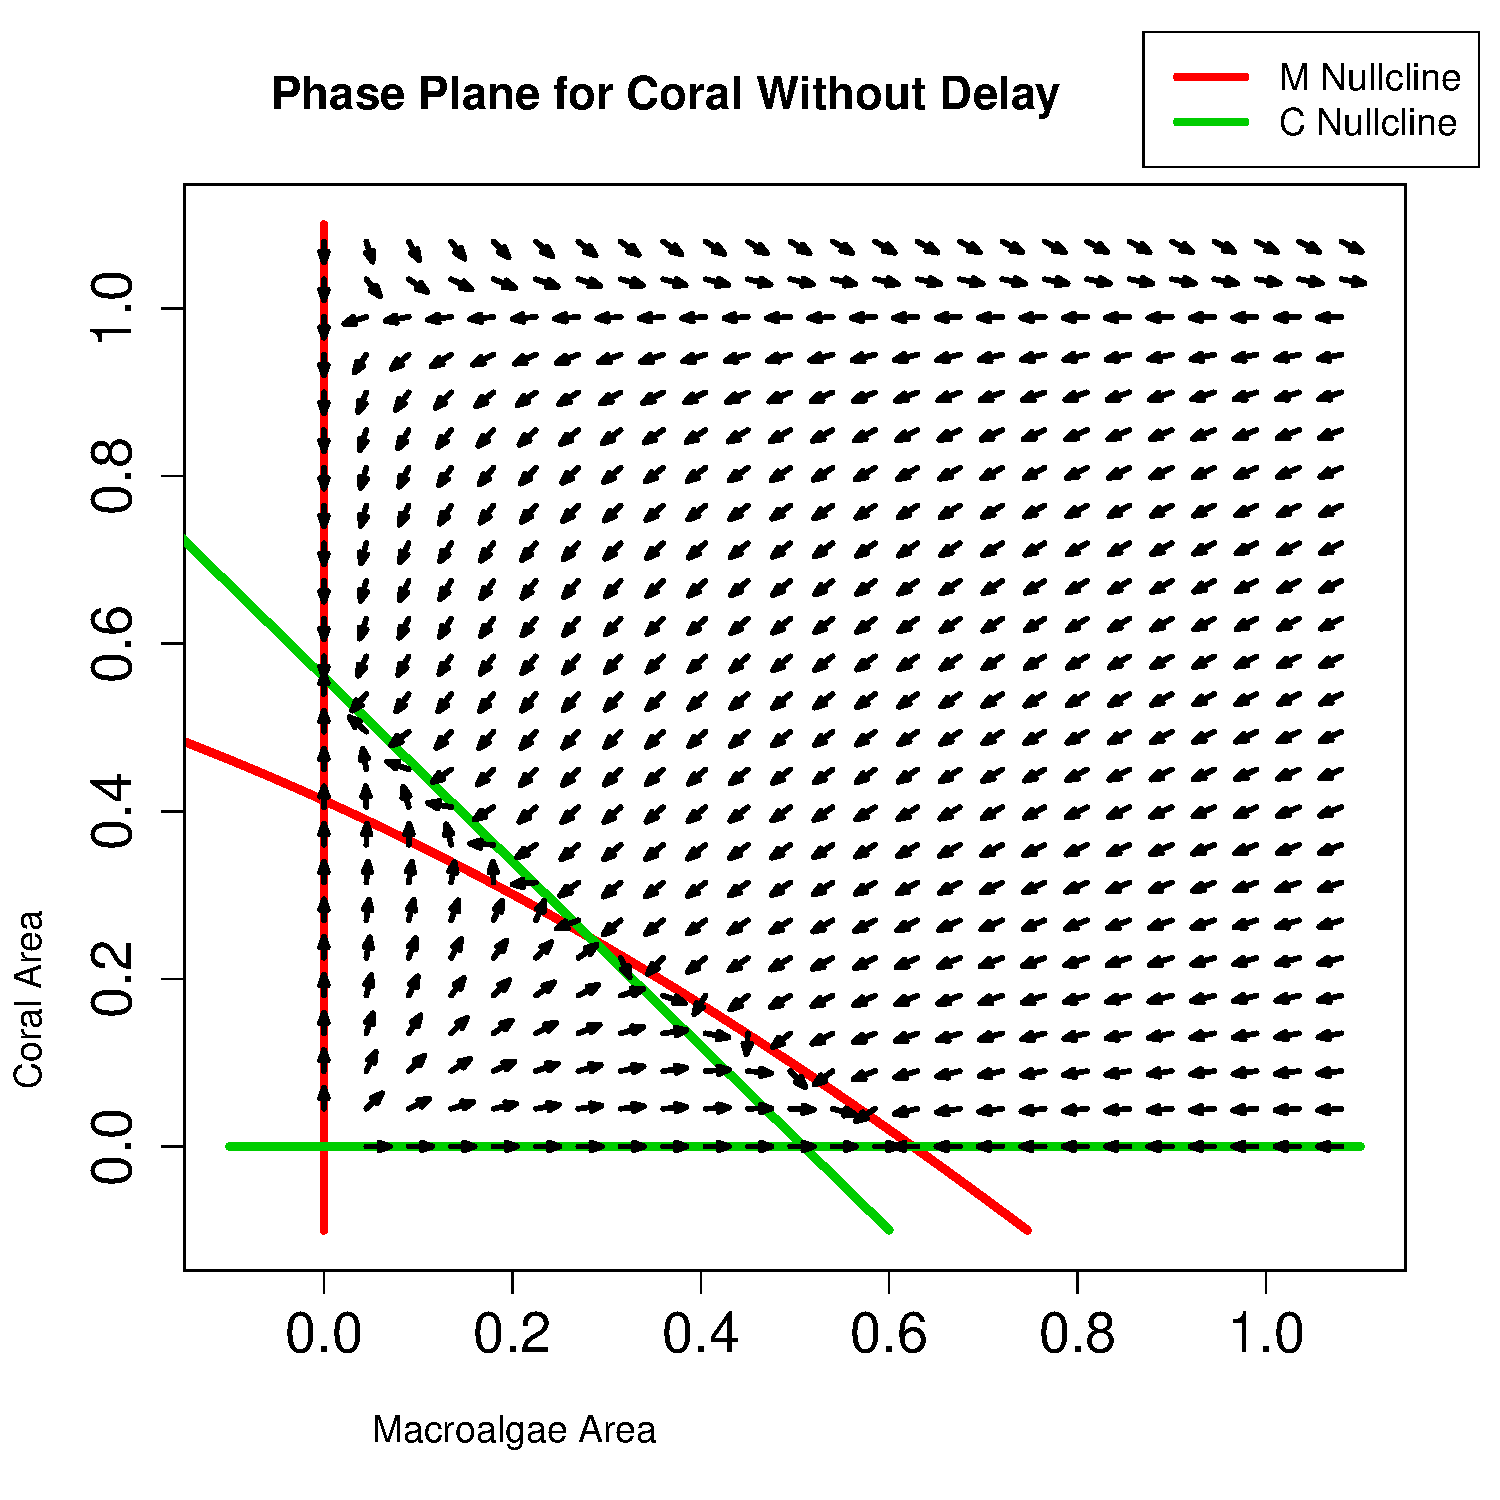
\includegraphics[scale=.325]{./nullclines.pdf}

\end{frame}


\begin{frame}{Initial Conditions}
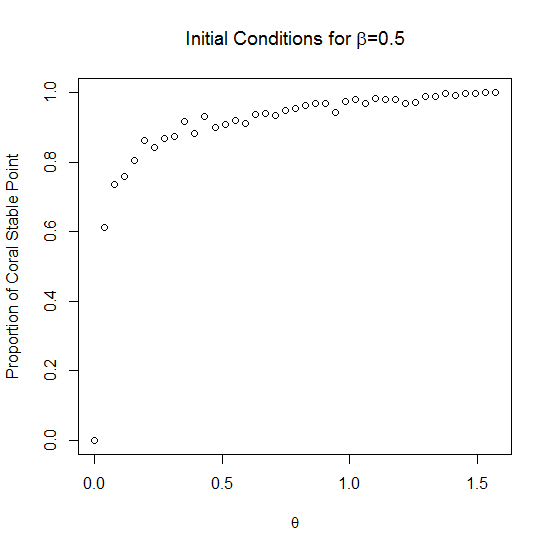
\includegraphics[scale=.425]{ic.png}
\end{frame}

\begin{frame}{The Three Models}
Based on the plot, we will try the following three models
\begin{itemize}
\item Binomial Logit\\
Fits the model $logit(y)=a+bx$ where $logit(y)=log(\frac{y}{1-y})$\\
\item Poisson Log\\
Fits the model $log(y)=a+bx$\\
\item Ordinary Least Squares (OLS)\\
Fits the model $y=a+bx$\\
\end{itemize}
\end{frame}


\begin{frame}{Binomial Logit, Poisson Log, or OLS}
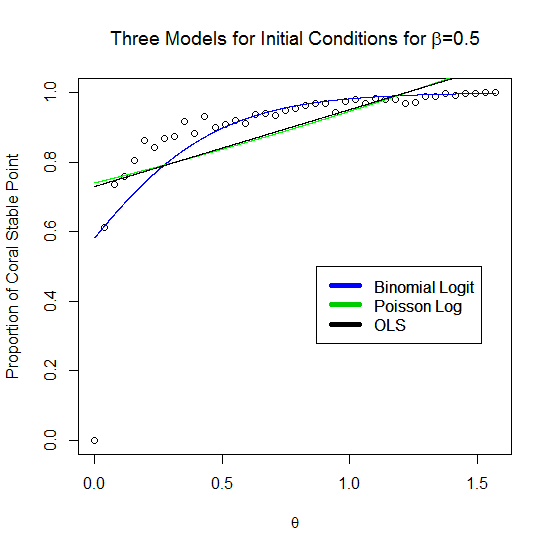
\includegraphics[scale=.425]{theta_three_models.png}
\end{frame}

\begin{frame}{The Binomial Logit Model}
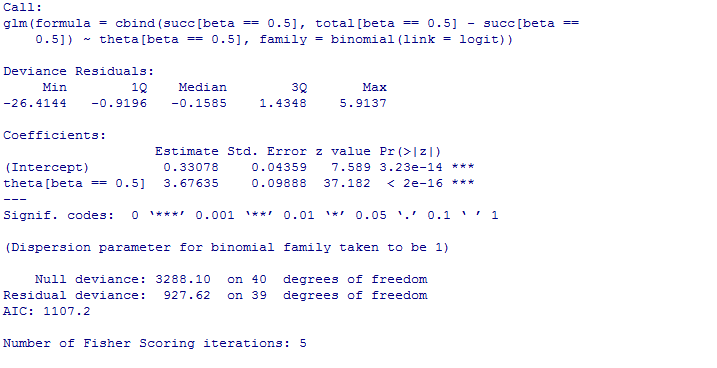
\includegraphics[scale=.5]{theta_logit_summary.png}\\
A goodness of fit test: $P(\chi^{2}_{1}>3288.10-927.62)$\\
Do the same thing for the Poisson and OLS\\
Test beta and tau\\
Do interaction terms\\
\end{frame}


%%% Local Variables:
%%% mode: latex
%%% TeX-master: "Presentation2"
%%% End:
